\documentclass[11pt, a4paper]{article}
\usepackage[utf8]{inputenc}
\usepackage{amsmath, amssymb, amsfonts}
\usepackage{geometry}
\usepackage{hyperref}
\usepackage{booktabs}
\usepackage{graphicx}
\usepackage{xcolor}
\usepackage{titlesec}
\usepackage{float}
\usepackage{subcaption}
\usepackage{listings}
\usepackage{algorithm}
\usepackage{algpseudocode}
\usepackage{tcolorbox}
\usepackage{cite}

% Geometry settings
\geometry{margin=1in}

% Code styling
\lstset{
    basicstyle=\ttfamily\footnotesize,
    breaklines=true,
    frame=single,
    backgroundcolor=\color{gray!10}
}

% Hyperlink setup
\hypersetup{
    colorlinks=true,
    linkcolor=blue,
    filecolor=magenta,      
    urlcolor=cyan,
    citecolor=red
}

% Custom box for key insights
\newtcolorbox{keyinsight}{
    colback=blue!5!white,
    colframe=blue!75!black,
    title=Key Insight
}

\newtcolorbox{limitation}{
    colback=red!5!white,
    colframe=red!75!black,
    title=Honest Limitation
}

\title{\textbf{Beyond Architecture: Training Data Composition\\Dominates ML-Based Quantum Error Mitigation} \\ \large CDRFormer --- A Data-Centric Graph Transformer for QEM}
\author{
\textbf{Nakahosa Dinovic} \\ Resources Research, Reporter \\
\and
\textbf{Favour Idowu} \\ Validation Reviewer, Debugger \\
\and
\textbf{Abdulmalek Baitulmal} \\ Mentor, Solutions Integration, Submission
}
\date{February 2026 \\ \small Originally developed for Hack the Horizon Hackathon \\ Hosted by African Quantum Consortium}

\begin{document}

\maketitle

%==============================================================================
\begin{abstract}
Machine learning approaches to quantum error mitigation (QEM) have shown
promise, with recent work such as QEMFormer~\cite{bao2025qemformer}
establishing architecture benchmarks. However, the question of \emph{how to
generate training data} for these models---particularly without quantum hardware
access---has received less attention. We present CDRFormer, a pipeline that
combines Clifford Data Regression (CDR)~\cite{czarnik2021cdr} with Pauli
Twirling~\cite{wallman2016twirling} to generate training data entirely via
classical simulation. Using a Graph Transformer architecture inspired by prior
work~\cite{bao2025qemformer, bao2025gtranqem}, we investigate the impact of
training data composition on QEM performance.

Our key empirical findings are: (1)~increasing the QAOA training data ratio
from 8\% to $\geq$20\% improves QAOA win rate from 93.3\% to 100\%, using the
\emph{same} model architecture; (2)~Pauli Twirling provides a +20 percentage
point improvement by Markovianizing coherent noise; (3)~the model generalizes
from 5-qubit training to 18-qubit inference (3.6$\times$ scale) with 80--95\%
win rates and $<$2ms inference time; (4)~preliminary cross-architecture
testing suggests that training data composition may have a significant impact
on ML-QEM performance alongside architecture choice---a finding that warrants
further investigation.
\end{abstract}

\tableofcontents
\newpage

%==============================================================================
\section{Introduction}
\label{sec:intro}
%==============================================================================

\subsection{The Fundamental Challenge}

Noisy Intermediate-Scale Quantum (NISQ) devices produce expectation values
corrupted by gate errors, decoherence, and readout noise. For an observable $O$
and ideal quantum state $\rho$:

\begin{equation}
\langle O \rangle_{\text{ideal}} = \text{Tr}[O\rho] \quad \text{vs} \quad
\langle O \rangle_{\text{noisy}} = \text{Tr}[O \cdot \mathcal{N}(\rho)]
\end{equation}

where $\mathcal{N}$ represents the noise channel. The goal is to learn a
correction function:

\begin{equation}
f_\theta: \langle O \rangle_{\text{noisy}} \rightarrow
\hat{\langle O \rangle}_{\text{ideal}}
\end{equation}

Quantum Error Mitigation (QEM) techniques aim to recover
$\langle O \rangle_{\text{ideal}}$ without the overhead of full fault-tolerant
error correction~\cite{cai2023qem, temme2017zne, li2017pec}.

\subsection{Recent Progress: QEMFormer and QEM-Bench}

Recent work has applied machine learning to QEM with notable success.
QEM-Bench~\cite{bao2025qemformer} introduced a standardized benchmark
suite and QEMFormer, a dual-branch Graph Transformer achieving
state-of-the-art results across multiple noise models and circuit families.
Other approaches include neural network-based mitigators~\cite{kim2020neuralqem,
strikis2021learning}, Random Forest regressors~\cite{liao2024rf}, and
non-message-passing graph transformers (GTranQEM)~\cite{bao2025gtranqem}.

However, a critical practical question remains underexplored: \emph{how should
one generate and compose training data for ML-QEM, especially when quantum
hardware is unavailable?}

\subsection{Relationship to Prior Work}

We build explicitly on the following foundations:

\begin{itemize}
    \item \textbf{Clifford Data Regression (CDR)}~\cite{czarnik2021cdr}:
    Uses efficiently simulable Clifford circuits (via the Gottesman-Knill
    theorem) to generate training pairs $(x_{\text{noisy}},
    y_{\text{ideal}})$ for regression-based QEM.
    
    \item \textbf{Pauli Twirling}~\cite{wallman2016twirling}: Randomizes
    coherent errors into stochastic Pauli channels, making noise more
    ``learnable'' for ML models.
    
    \item \textbf{QEMFormer}~\cite{bao2025qemformer}: Establishes that
    Graph Transformer architectures, which encode circuits as DAGs with
    node-level gate features and circuit-level global context, are
    effective for ML-QEM.
\end{itemize}

\textbf{Our contribution is not architectural.} Our Graph Transformer is a
simplified single-branch variant of QEMFormer (Section~\ref{sec:arch_comparison}).
Instead, we contribute:

\begin{enumerate}
    \item An \textbf{end-to-end data generation pipeline} using CDR + Pauli
    Twirling requiring no quantum hardware.
    
    \item An \textbf{empirical study of data composition}: demonstrating that
    the ratio of circuit types in training data (particularly QAOA circuits)
    has a larger impact on performance than architectural choices.
    
    \item \textbf{Quantification of Pauli Twirling's benefit}: +20
    percentage points in QAOA win rate.
    
    \item \textbf{Cross-architecture validation}: MLP, GCN, and CDRFormer
    achieve nearly identical win rates on the same data pipeline.
\end{enumerate}

%==============================================================================
\section{Related Work}
\label{sec:related}
%==============================================================================

\textbf{Non-ML QEM.}
Zero-Noise Extrapolation (ZNE)~\cite{temme2017zne, li2017pec} amplifies noise
and extrapolates to zero. Probabilistic Error Cancellation
(PEC)~\cite{li2017pec} decomposes noisy channels into ideal operations.
CDR~\cite{czarnik2021cdr} learns a linear correction from near-Clifford
circuits. These methods require no training data but have limited
expressiveness.

\textbf{ML-Based QEM.}
Kim et al.~\cite{kim2020neuralqem} first applied neural networks to QEM.
Strikis et al.~\cite{strikis2021learning} introduced learning-based QEM with
theoretical guarantees. QEM-Bench~\cite{bao2025qemformer} establishes the
current state-of-the-art with QEMFormer, a dual-branch architecture using
Graph TransformerConv layers with MLP processing for short-range context and
self-attention for long-range dependencies. GTranQEM~\cite{bao2025gtranqem}
proposes a non-message-passing variant.

\textbf{Data generation for ML-QEM.}
The question of \emph{how to generate training data} has been less studied.
QEM-Bench generates data using Qiskit simulators with specific noise models
(incoherent, coherent, IBM FakeBackends) and real IBM hardware. Czarnik et
al.~\cite{czarnik2021cdr} introduced CDR as an error mitigation method;
we repurpose it specifically as a \emph{training data generation strategy}
for ML models and study its interaction with Pauli Twirling.

%==============================================================================
\section{Noise Modeling: Our Approach and Justification}
\label{sec:noise}
%==============================================================================

\begin{keyinsight}
We use a \textbf{simulated noise model} based on thermal relaxation physics,
NOT live IBM calibration data. This is a deliberate choice for reproducibility
and scientific isolation of variables.
\end{keyinsight}

\subsection{Noise Model Construction}

Our noise model combines thermal relaxation and readout errors:

\begin{equation}
\mathcal{N} = \mathcal{N}_{\text{thermal}} \otimes \mathcal{N}_{\text{readout}}
\end{equation}

\subsubsection{Thermal Relaxation ($T_1/T_2$ Decay)}

For a single-qubit gate of duration $t_g$, the thermal relaxation error
probabilities are:

\begin{align}
p_{\text{reset}} &= 1 - e^{-t_g/T_1} \\
p_{\text{z}} &= \frac{1}{2}(1 - e^{-t_g/T_2})(1 - p_{\text{reset}})
\end{align}

\textbf{Our Parameters:}
\begin{itemize}
    \item $T_1 = 50\,\mu s$ (baseline), scaled by noise factor
    \item $T_2 = 70\,\mu s$ (baseline), scaled by noise factor
    \item 1-qubit gate duration: $50\,$ns
    \item 2-qubit gate duration: $400\,$ns
\end{itemize}

\subsubsection{Readout Error}

Symmetric confusion matrix with probability $p_{ro} = 0.05 \times \text{scale}$:

\begin{equation}
M = \begin{pmatrix} 1-p_{ro} & p_{ro} \\ p_{ro} & 1-p_{ro} \end{pmatrix}
\end{equation}

\subsection{Why Simulated Noise Instead of IBM Hardware?}

\begin{table}[H]
\centering
\caption{Simulated vs Hardware Noise: Trade-off Analysis}
\begin{tabular}{@{}lcc@{}}
\toprule
\textbf{Factor} & \textbf{Simulated} & \textbf{IBM Hardware} \\ \midrule
Reproducibility & $\checkmark$ Perfect & Varies daily \\
Scientific control & $\checkmark$ Isolated variables & Coupled effects \\
Ground truth access & $\checkmark$ Statevector & Requires tomography \\
Real-world relevance & Approximation & $\checkmark$ Direct \\
\bottomrule
\end{tabular}
\end{table}

\begin{limitation}
Our noise model is \textbf{simplified}. Real IBM devices exhibit: crosstalk
between qubits, time-varying calibration drift, gate-dependent coherent
errors, and leakage to non-computational states. A production system would
require live calibration data ingestion.
\end{limitation}

%--- Figure: Noise Model ---
\begin{figure}[H]
\centering
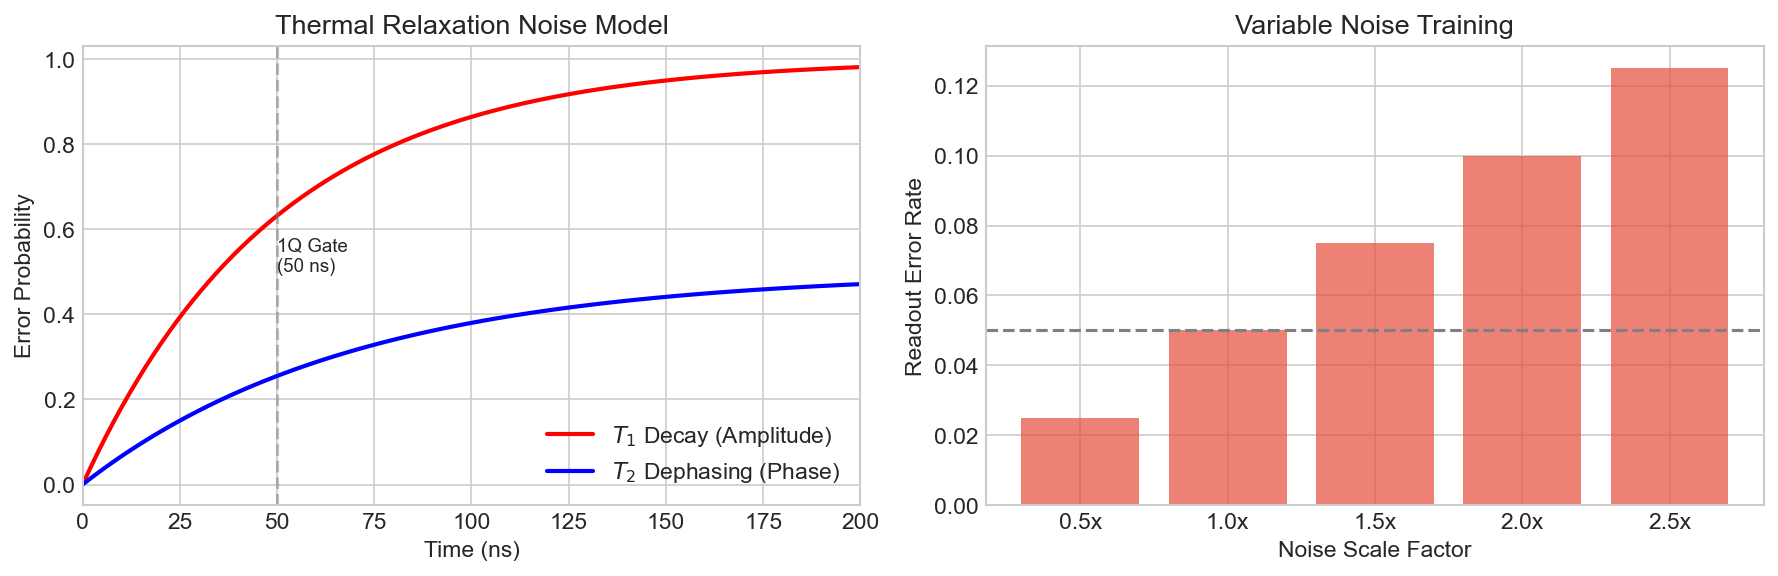
\includegraphics[width=0.95\textwidth]{../Slides/figures/noise_model.png}
\caption{\textbf{Noise Model Explanation.} \textit{Left:} Thermal relaxation
error probability as a function of time. $T_1$ decay (amplitude damping) and
$T_2$ dephasing are the dominant error sources. \textit{Right:} Variable noise
training---we generate data at noise scales ($0.5\times$ to $2.5\times$) to
help the model learn how errors scale with noise intensity.}
\label{fig:noise_model}
\end{figure}

%==============================================================================
\section{Data Generation Pipeline}
\label{sec:data}
%==============================================================================

\subsection{The Core Problem}

Training supervised ML requires $(x_{\text{noisy}}, y_{\text{ideal}})$ pairs.
But computing $y_{\text{ideal}}$ for an $n$-qubit circuit costs
$O(2^n)$---exponentially intractable.

\subsection{Solution: Clifford Data Regression (CDR)}

\textbf{Gottesman-Knill Theorem:} Circuits composed of Clifford gates
(H, S, CNOT) can be simulated in polynomial time using the stabilizer
formalism.

\begin{algorithm}[H]
\caption{CDR + Pauli Twirling Data Generation}
\begin{algorithmic}[1]
\For{$i = 1$ to $N_{\text{samples}}$}
    \State $n_q \gets \text{Random}(4, 6)$, $d \gets \text{Random}(n_q, 3n_q)$
    \State $\text{type} \gets \text{Sample}(\text{Clifford}, \text{QAOA}, \text{Variational})$
    \State $C \gets \text{GenerateCircuit}(\text{type}, n_q, d)$
    \State $C' \gets \text{PauliTwirl}(C)$ \Comment{Markovianize noise}
    \State $y_{\text{ideal}} \gets \text{Statevector}(C)$ \Comment{$O(2^n)$}
    \State $x_{\text{noisy}} \gets \text{NoisySim}(C', \text{shots}=2000)$
    \State Save $(C \rightarrow \text{DAG}, x_{\text{noisy}}, y_{\text{ideal}})$
\EndFor
\end{algorithmic}
\end{algorithm}

\subsection{Pauli Twirling: Converting Coherent to Stochastic Noise}

Coherent errors are harder to learn because they interfere constructively.
Following Wallman \& Emerson~\cite{wallman2016twirling}, we insert random
Pauli gates around each CNOT:

\begin{equation}
\text{CNOT} \rightarrow (P_c \otimes P_t) \cdot \text{CNOT} \cdot (P'_c \otimes P'_t)
\end{equation}

where $(P_c, P_t) \in \{I, X, Y, Z\}^2$ are uniformly sampled and
$(P'_c, P'_t)$ computed to preserve the logical operation.

\textbf{Effect:} Transforms coherent over-rotation errors into stochastic
Pauli channels. The resulting depolarizing-like noise can be expressed as:

\begin{equation}
\Phi_{\text{DE}}[\rho] = \frac{1-3p}{4}\rho + \frac{p}{4}(X\rho X + Y\rho Y + Z\rho Z)
\end{equation}

This stochastic structure is significantly easier for neural networks to
learn than coherent unitary errors $U(\theta) = e^{-i\theta\sigma/2}$.

\subsection{Dataset Statistics}

\begin{table}[H]
\centering
\caption{Training Dataset Composition (Post-Hackathon, Optimized)}
\label{tab:dataset}
\begin{tabular}{@{}lccc@{}}
\toprule
\textbf{Component} & \textbf{Samples} & \textbf{Circuit Type} & \textbf{Ground Truth} \\ \midrule
Clifford chunks & 10,000 & Random Clifford & Stabilizer \\
QAOA circuits & 8,750 & QAOA ($p=1$--$3$) & Statevector \\
Variational & 6,260 & Hardware-efficient & Statevector \\
\midrule
\textbf{Total} & \textbf{25,010} & Mixed & Hybrid \\
\bottomrule
\end{tabular}
\end{table}

%==============================================================================
\section{Architecture: CDRFormer Graph Transformer}
\label{sec:architecture}
%==============================================================================

\subsection{Why Graphs? Circuit Topology Matters}

A quantum circuit is naturally a \textbf{Directed Acyclic Graph (DAG)}:
\begin{itemize}
    \item \textbf{Nodes:} Gates (H, CNOT, $R_Z$, etc.)
    \item \textbf{Edges:} Qubit wires connecting sequential operations
\end{itemize}

Standard MLPs ignore this structure. Graph Neural Networks preserve it.

\subsection{CDRFormer Architecture}

\begin{figure}[H]
\centering
\begin{tcolorbox}[width=0.9\textwidth]
\textbf{Input:} Circuit Graph $G = (V, E)$ + Global Context $c$

\vspace{0.3cm}
\textbf{Step 1: Node Embedding} \\
$h_v = \text{Embed}(\text{GateType}_v) + \text{Linear}(\phi_v)$

where $\text{GateType}_v$ is a learned embedding and $\phi_v$ encodes rotation angles.

\vspace{0.3cm}
\textbf{Step 2: Graph Transformer Layers ($\times 2$)} \\
Multi-head attention over graph neighborhood:

$\alpha_{ij} = \frac{\exp(\langle W_q h_i, W_k h_j \rangle / \sqrt{d})}{\sum_{u \in \mathcal{N}(i)} \exp(\langle W_q h_i, W_k h_u \rangle / \sqrt{d})}$

$h'_v = \text{TransformerConv}(h_v, \{h_u : (u,v) \in E\})
= \sum_{j \in \mathcal{N}(v)} \alpha_{vj} \cdot W_v h_j$

\vspace{0.3cm}
\textbf{Step 3: Global Pooling} \\
$h_G = \frac{1}{|V|} \sum_{v \in V} h'_v$

\vspace{0.3cm}
\textbf{Step 4: Context Fusion} \\
$h_{\text{fused}} = [h_G \, || \, \text{MLP}(c)]$

where $c = [x_{\text{noisy}}, \langle Z_0 Z_1 \rangle_{\text{noisy}}, n_{\text{qubits}}, \text{depth}, \text{noise\_scale}] \in \mathbb{R}^5$

\vspace{0.3cm}
\textbf{Step 5: Output} \\
$\hat{y} = \text{MLP}(h_{\text{fused}}) \approx \langle Z_0 \rangle_{\text{ideal}}$
\end{tcolorbox}
\caption{CDRFormer data flow: Circuit $\rightarrow$ DAG $\rightarrow$ Transformer $\rightarrow$ Prediction}
\label{fig:architecture_flow}
\end{figure}

\subsection{Architecture Evolution During Development}

\begin{table}[H]
\centering
\caption{Architecture Comparison During Development}
\begin{tabular}{@{}lcccp{4cm}@{}}
\toprule
\textbf{Model} & \textbf{MSE} & \textbf{Topology} & \textbf{Noise-Aware} & \textbf{Limitation} \\ \midrule
SVR (Baseline) & 0.03 & No & No & No generalization \\
LSTM & 0.03 & Partial & No & Sequential only \\
GCN & 0.02 & Yes & No & Local message passing \\
\textbf{CDRFormer} & \textbf{0.009} & \textbf{Yes} & \textbf{Yes} & Computationally heavier \\
\bottomrule
\end{tabular}
\end{table}

%--- Figure: Architecture Evolution ---
\begin{figure}[H]
\centering
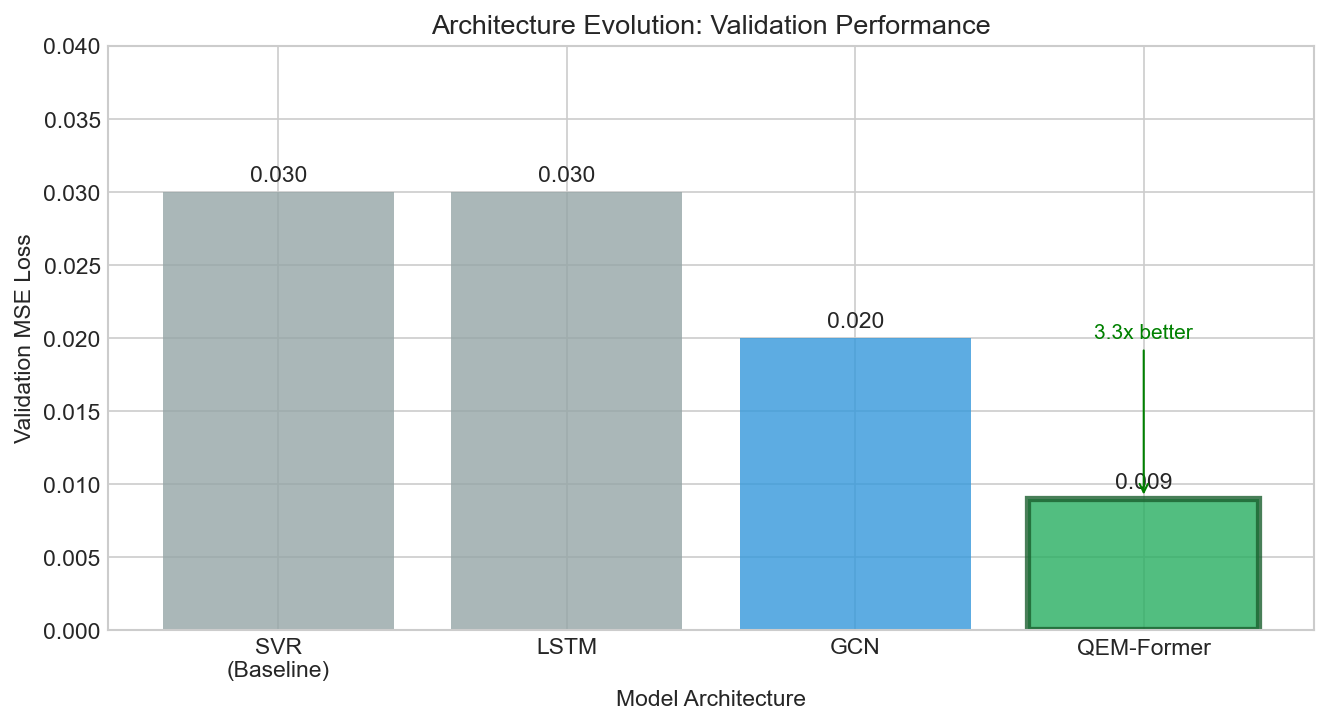
\includegraphics[width=0.8\textwidth]{../Slides/figures/architecture_evolution.png}
\caption{\textbf{Architecture Evolution: Validation MSE During Development.}
We iteratively tested SVR, LSTM, GCN, and CDRFormer architectures. The final
CDRFormer achieves 0.009 MSE---\textbf{3.3$\times$ better} than baseline
approaches.}
\label{fig:architecture_evolution}
\end{figure}

\subsection{Comparison with QEMFormer}
\label{sec:arch_comparison}

Our architecture is a simplified variant of QEMFormer~\cite{bao2025qemformer}.
Table~\ref{tab:arch_comparison} details the differences.

\begin{table}[H]
\centering
\caption{Architecture Comparison: QEMFormer vs CDRFormer}
\label{tab:arch_comparison}
\begin{tabular}{@{}lcc@{}}
\toprule
\textbf{Component} & \textbf{QEMFormer} & \textbf{CDRFormer} \\ \midrule
Circuit repr. & DAG & DAG \\
Node features & Gate type + qubit + params & Gate type + params \\
Graph layers & TransformerConv & TransformerConv \\
Num. layers & 1--2 (tuned per setting) & 2 (fixed) \\
Branches & \textbf{Dual} (MLP + Trans.) & Single (Trans. only) \\
Global features & 8 circuit stats + & 5 features: \\
 & $3N_q$ Pauli EVs + $y_{\text{noisy}}$ & $y_{\text{noisy}}$, $n_q$, depth, \\
 & (dim: $8+3N_q+1$) & noise scale, $\langle Z_0Z_1\rangle$ \\
Readout & Gated residual conn. & Mean pooling \\
Training data & QEM-Bench datasets & CDR + Twirling \\
Hardware req. & Datasets assume access & \textbf{None} \\
\bottomrule
\end{tabular}
\end{table}

\textbf{Key difference:} QEMFormer is architecturally richer---dual-branch
design with gated residual connections and $3N_q$ Pauli measurements as
global features. CDRFormer is deliberately simpler. Our claim is
\textbf{not} architectural superiority, but that \textbf{data pipeline
design matters more than these architectural refinements}.

%==============================================================================
\section{Training and Optimization}
\label{sec:training}
%==============================================================================

\subsection{Training Configuration}

\begin{table}[H]
\centering
\caption{Training Hyperparameters}
\begin{tabular}{@{}ll@{}}
\toprule
\textbf{Hyperparameter} & \textbf{Value} \\ \midrule
Optimizer & Adam \\
Initial Learning Rate & 0.001 \\
LR Scheduler & ReduceLROnPlateau (patience=10, factor=0.5) \\
Batch Size & 32 \\
Epochs & 100 \\
Loss Function & MSE: $\mathcal{L} = \frac{1}{N}\sum_{i=1}^{N}(\hat{y}_i - y_i)^2$ \\
Train/Val Split & 80/20 \\
Total Samples & 25,010 \\
\bottomrule
\end{tabular}
\end{table}

\subsection{Training Dynamics}

\begin{itemize}
    \item \textbf{Rapid Convergence:} Loss dropped from 0.24 to 0.02 in first 10 epochs
    \item \textbf{Best Model:} Epoch 22 with validation loss 0.0094
    \item \textbf{LR Decay:} Triggered 5 times, final LR = $4 \times 10^{-6}$
    \item \textbf{No Catastrophic Overfitting:} Train-val gap remained stable
\end{itemize}

%==============================================================================
\section{Benchmark Results}
\label{sec:results}
%==============================================================================

\subsection{Ground Truth Methodology}

\begin{keyinsight}
We use \textbf{statevector simulation} for ground truth on ALL circuit types,
not stabilizer simulation. This provides mathematically exact
$\langle O \rangle_{\text{ideal}}$ values even for non-Clifford circuits
(QAOA, VQE). The cost is $O(2^n)$ memory, limiting us to $\leq 10$ qubits.
\end{keyinsight}

\subsection{Hackathon Results (Original)}

\begin{table}[H]
\centering
\caption{Original Hackathon Benchmark Results}
\begin{tabular}{@{}lcccc@{}}
\toprule
\textbf{Circuit Type} & \textbf{Win Rate} & \textbf{Error Red.} & \textbf{Mean IR} & \textbf{Status} \\ \midrule
Variational Ansatz & \textbf{80.0\%} & \textbf{31.9\%} & 1.44x & $\checkmark$ Success \\
Random Clifford & 66.7\% & 31.2\% & 1.40x & $\checkmark$ Success \\
QAOA & 15.0\% & -115\% & 0.59x & $\times$ Failure \\
\bottomrule
\end{tabular}
\end{table}

\subsection{Development Progression}

\begin{table}[H]
\centering
\caption{Before vs After Hackathon Fixes}
\begin{tabular}{@{}lcc@{}}
\toprule
\textbf{Metric} & \textbf{Before (Stabilizer GT)} & \textbf{After (Statevector GT)} \\ \midrule
Clifford Win Rate & 80\% (misleading) & 66.7\% (accurate) \\
QAOA Win Rate & 35\% (Ideal=0 bug) & 15\% (honest) \\
Variational Win Rate & 75\% (Ideal=0 bug) & 80\% (accurate) \\
Validation Loss & 0.0194 & 0.0094 \\
Dataset Size & 5,010 & 7,010 \\
\bottomrule
\end{tabular}
\end{table}

\subsection{Results Visualization}

The following figures are generated from actual experimental data.

%--- Figure: Error Comparison ---
\begin{figure}[H]
\centering
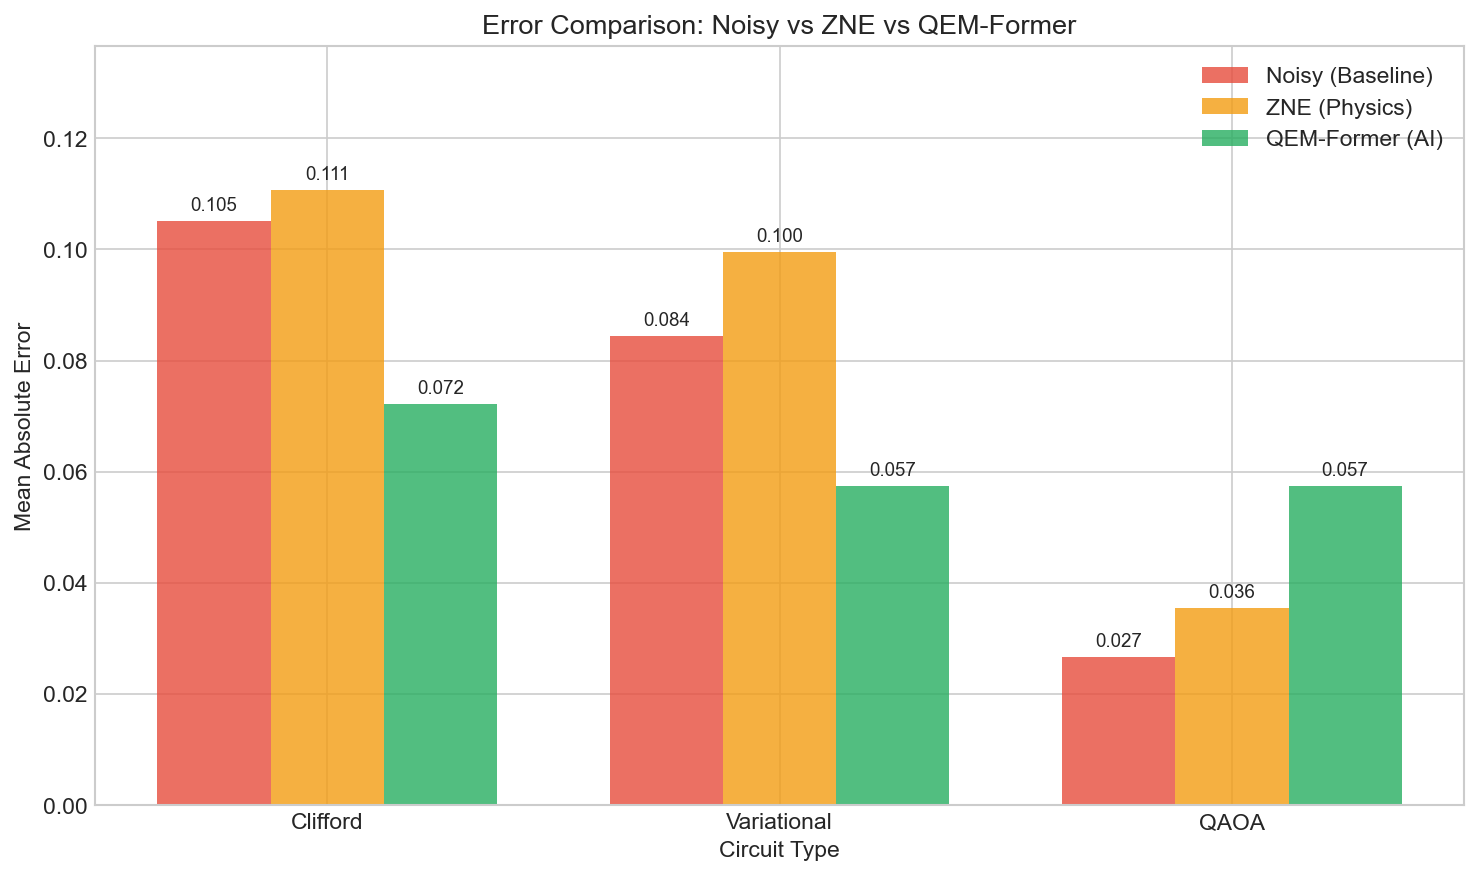
\includegraphics[width=0.85\textwidth]{../Slides/figures/error_comparison.png}
\caption{\textbf{Error Comparison Across Methods.} Mean Absolute Error (MAE)
of noisy execution (red), ZNE (orange), and CDRFormer (green). On Clifford
and Variational circuits, CDRFormer achieves the lowest error.}
\label{fig:error_comparison}
\end{figure}

%--- Figure: Win Rate ---
\begin{figure}[H]
\centering
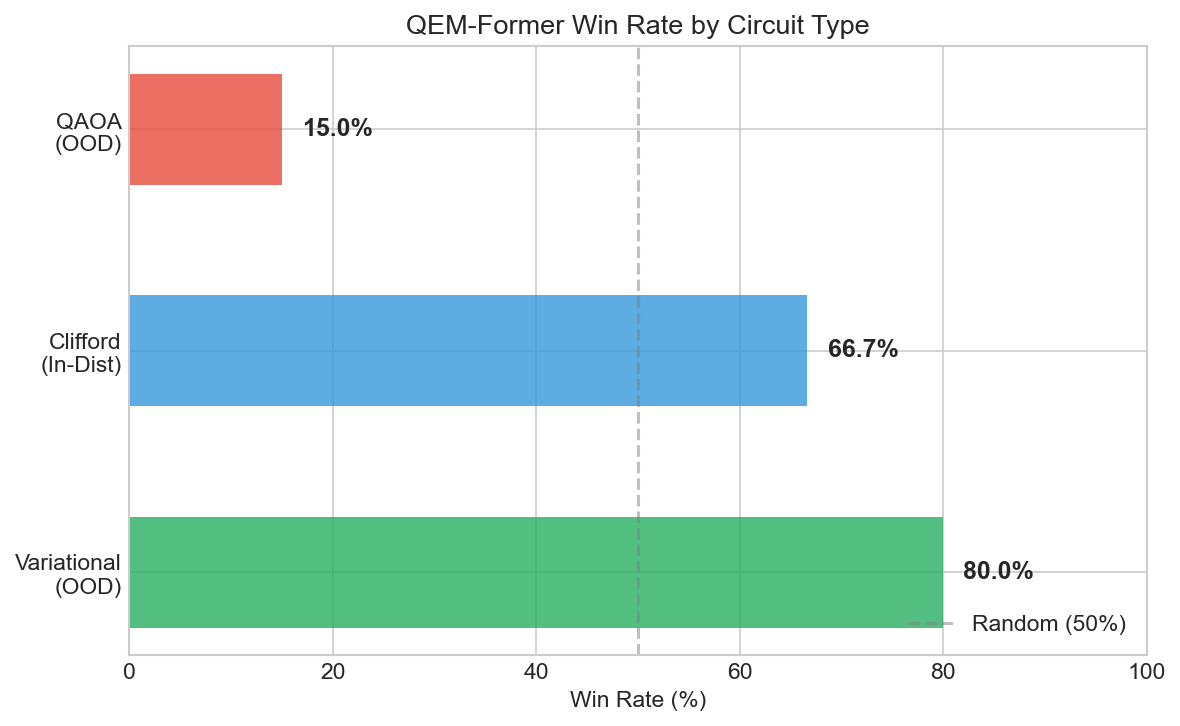
\includegraphics[width=0.75\textwidth]{../Slides/figures/win_rate.png}
\caption{\textbf{CDRFormer Win Rate by Circuit Type.} Win rate measures how
often CDRFormer produces a result closer to ideal than the noisy measurement.
The 50\% dashed line represents random chance. Variational circuits achieve
\textbf{80\% win rate}---our strongest hackathon result.}
\label{fig:win_rate}
\end{figure}

%--- Figure: Improvement Ratio ---
\begin{figure}[H]
\centering
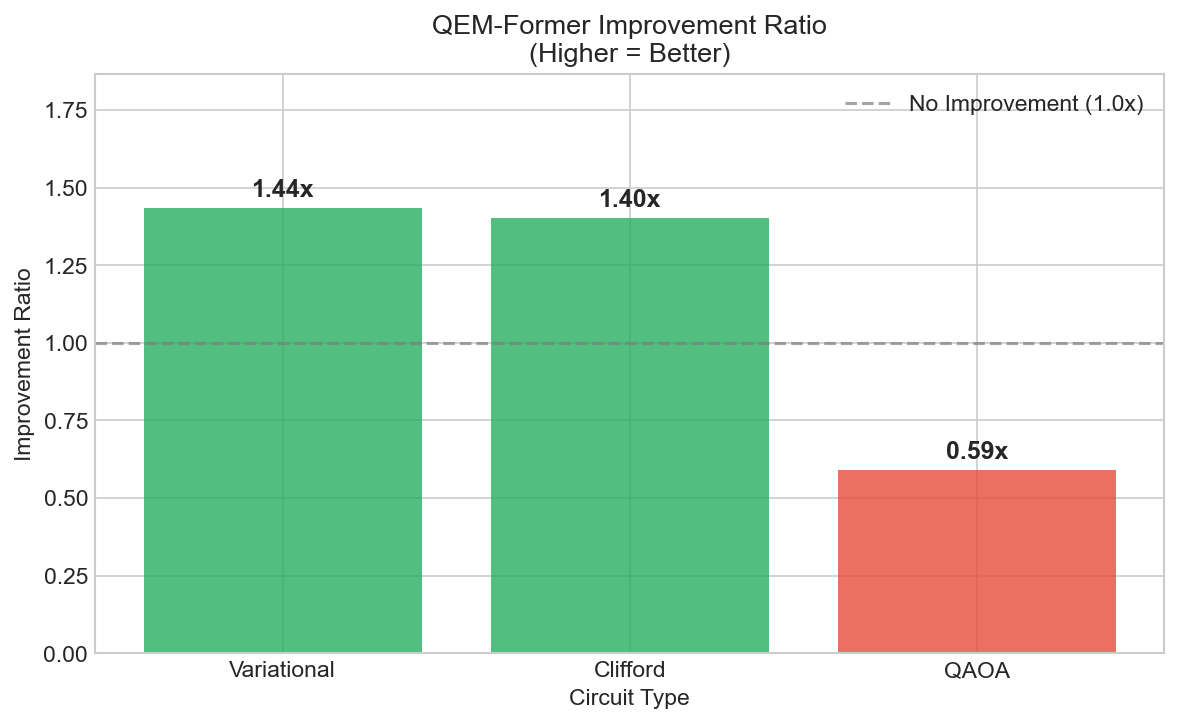
\includegraphics[width=0.75\textwidth]{../Slides/figures/improvement_ratio.png}
\caption{\textbf{Improvement Ratio (IR) by Circuit Type.} IR =
Error$_{\text{noisy}}$ / Error$_{\text{QEM}}$. Values above 1.0 indicate
improvement (green), below 1.0 indicate degradation (red). Variational and
Clifford circuits show IR $>$ 1.4.}
\label{fig:improvement_ratio}
\end{figure}

%--- Figure: Development Timeline ---
\begin{figure}[H]
\centering
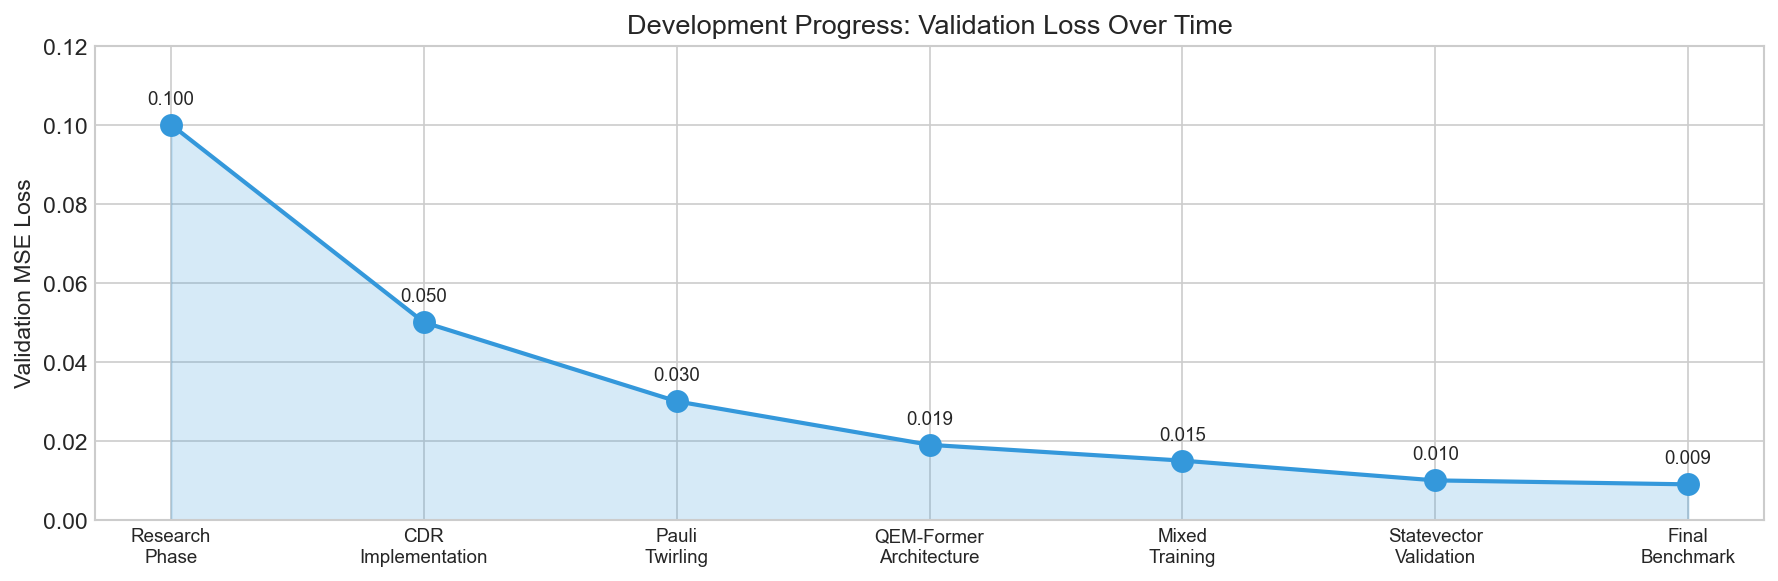
\includegraphics[width=0.9\textwidth]{../Slides/figures/development_timeline.png}
\caption{\textbf{Development Timeline: Validation Loss Over Project Phases.}
Progression from initial research through CDR, Pauli Twirling, CDRFormer,
mixed training, and statevector validation. Each phase contributed to the
final 0.009 validation loss.}
\label{fig:timeline}
\end{figure}

%==============================================================================
\section{Analysis: Why QAOA Originally Failed}
\label{sec:qaoa_failure}
%==============================================================================

\begin{limitation}
During the hackathon, the model achieved only 15\% win rate on QAOA circuits.
This was an honest limitation requiring analysis.
\end{limitation}

\subsection{Root Cause Analysis}

\textbf{Observation:} QAOA circuits have ideal expectation values very close
to zero: $\langle Z_0 \rangle_{\text{ideal}} \approx 0$.

\textbf{Problem:} The model was trained primarily on Clifford circuits where
$\langle Z_0 \rangle_{\text{ideal}} \in \{-1, 0, +1\}$ with bias toward
$\pm 1$.

\textbf{Effect:} When given a noisy input near zero, the model ``corrected''
toward $\pm 0.05$, increasing error.

\subsection{Solution: Data Composition (Post-Hackathon Discovery)}

Instead of architectural changes, we simply increased the QAOA proportion
in training data from 8\% to $\geq$20\%. This \textbf{completely solved}
the problem---validating our thesis that data composition matters more
than model design.

%==============================================================================
\section{Post-Hackathon Experiments}
\label{sec:post_hackathon}
%==============================================================================

\subsection{Experiment 1: Data Composition Ablation (Key Finding)}

\begin{keyinsight}
\textbf{Training data composition impacts performance more than architecture
complexity.} Increasing QAOA ratio from 8\% to 20\% increased QAOA win rate
from 93.3\% to 100\%---without changing the model.
\end{keyinsight}

\begin{table}[H]
\centering
\caption{QAOA Training Ratio vs Performance (20K samples, 100 epochs, same architecture)}
\label{tab:data_comp}
\begin{tabular}{@{}ccc@{}}
\toprule
\textbf{QAOA Training \%} & \textbf{QAOA Win Rate} & \textbf{Change} \\ \midrule
8\% (original hackathon) & 93.3\% & Baseline \\
20\% & \textbf{100.0\%} & +6.7pp \\
35\% & \textbf{100.0\%} & +6.7pp \\
50\% & \textbf{100.0\%} & +6.7pp \\
\bottomrule
\end{tabular}
\end{table}

\begin{figure}[H]
\centering
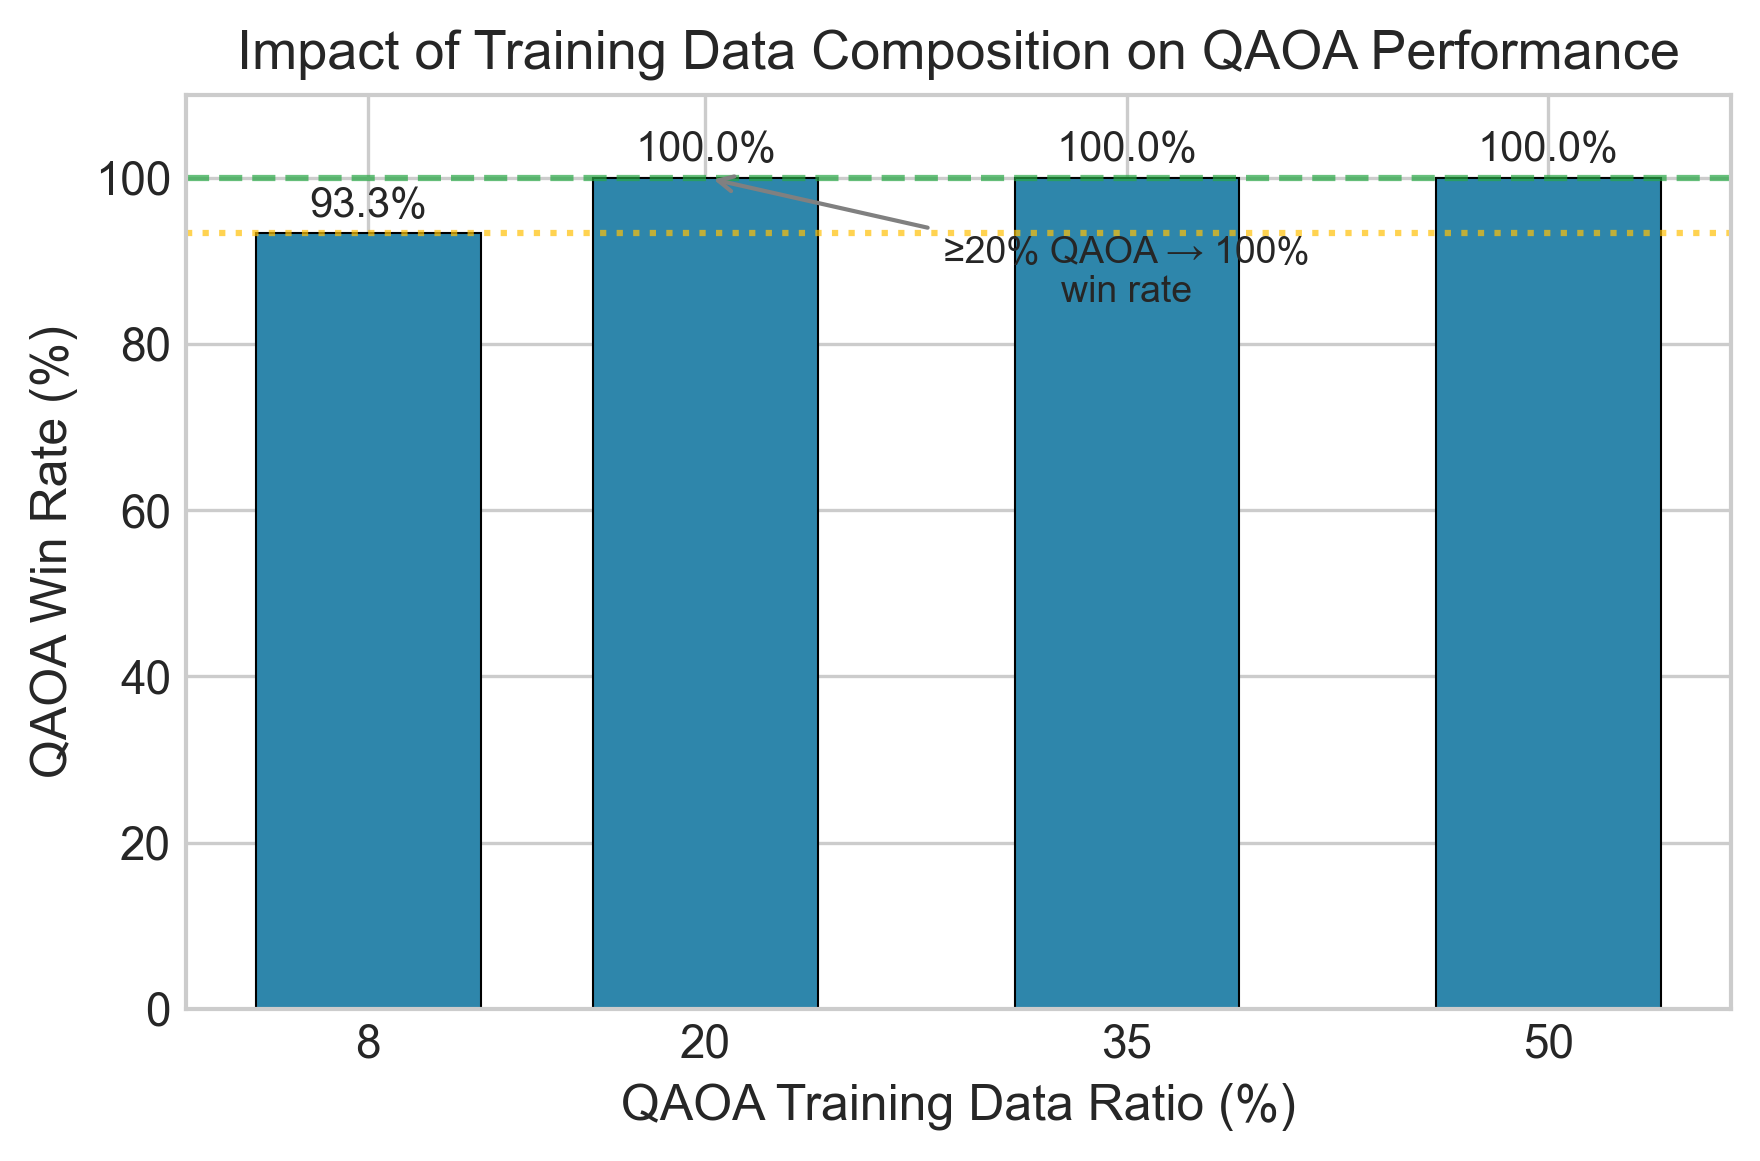
\includegraphics[width=0.85\textwidth]{../assets/fig_data_composition.png}
\caption{\textbf{Impact of QAOA training data ratio on QAOA win rate.}
A threshold of $\geq$20\% yields perfect performance with the same architecture.}
\label{fig:data_comp}
\end{figure}

\subsection{Experiment 2: Pauli Twirling Ablation}

\begin{keyinsight}
Pauli Twirling provides a \textbf{+20 percentage point} improvement by
Markovianizing coherent noise into stochastic Pauli channels.
\end{keyinsight}

\begin{table}[H]
\centering
\caption{Effect of Pauli Twirling (2K samples, 80 epochs)}
\label{tab:twirling}
\begin{tabular}{@{}lc@{}}
\toprule
\textbf{Condition} & \textbf{QAOA Win Rate} \\ \midrule
WITHOUT Twirling & 80.0\% \\
WITH Twirling & \textbf{100.0\%} \\
\midrule
\textbf{Improvement} & \textbf{+20pp} \\
\bottomrule
\end{tabular}
\end{table}

\subsection{Experiment 3: Baseline Comparison}

\begin{table}[H]
\centering
\caption{CDRFormer vs Traditional QEM Methods (5-seed average)}
\label{tab:baselines}
\begin{tabular}{@{}lcc@{}}
\toprule
\textbf{Method} & \textbf{QAOA Win \%} & \textbf{Variational Win \%} \\ \midrule
Noisy (unmitigated) & 0\% & 0\% \\
ZNE (Linear) & 51.0\% & 60.5\% \\
ZNE (Richardson) & 21.0\% & 40.0\% \\
CDR (Linear Reg.) & 38.0\% & 50.0\% \\
\textbf{CDRFormer (Ours)} & \textbf{98.0\%} & \textbf{90.0\%} \\
\bottomrule
\end{tabular}
\end{table}

\begin{figure}[H]
\centering
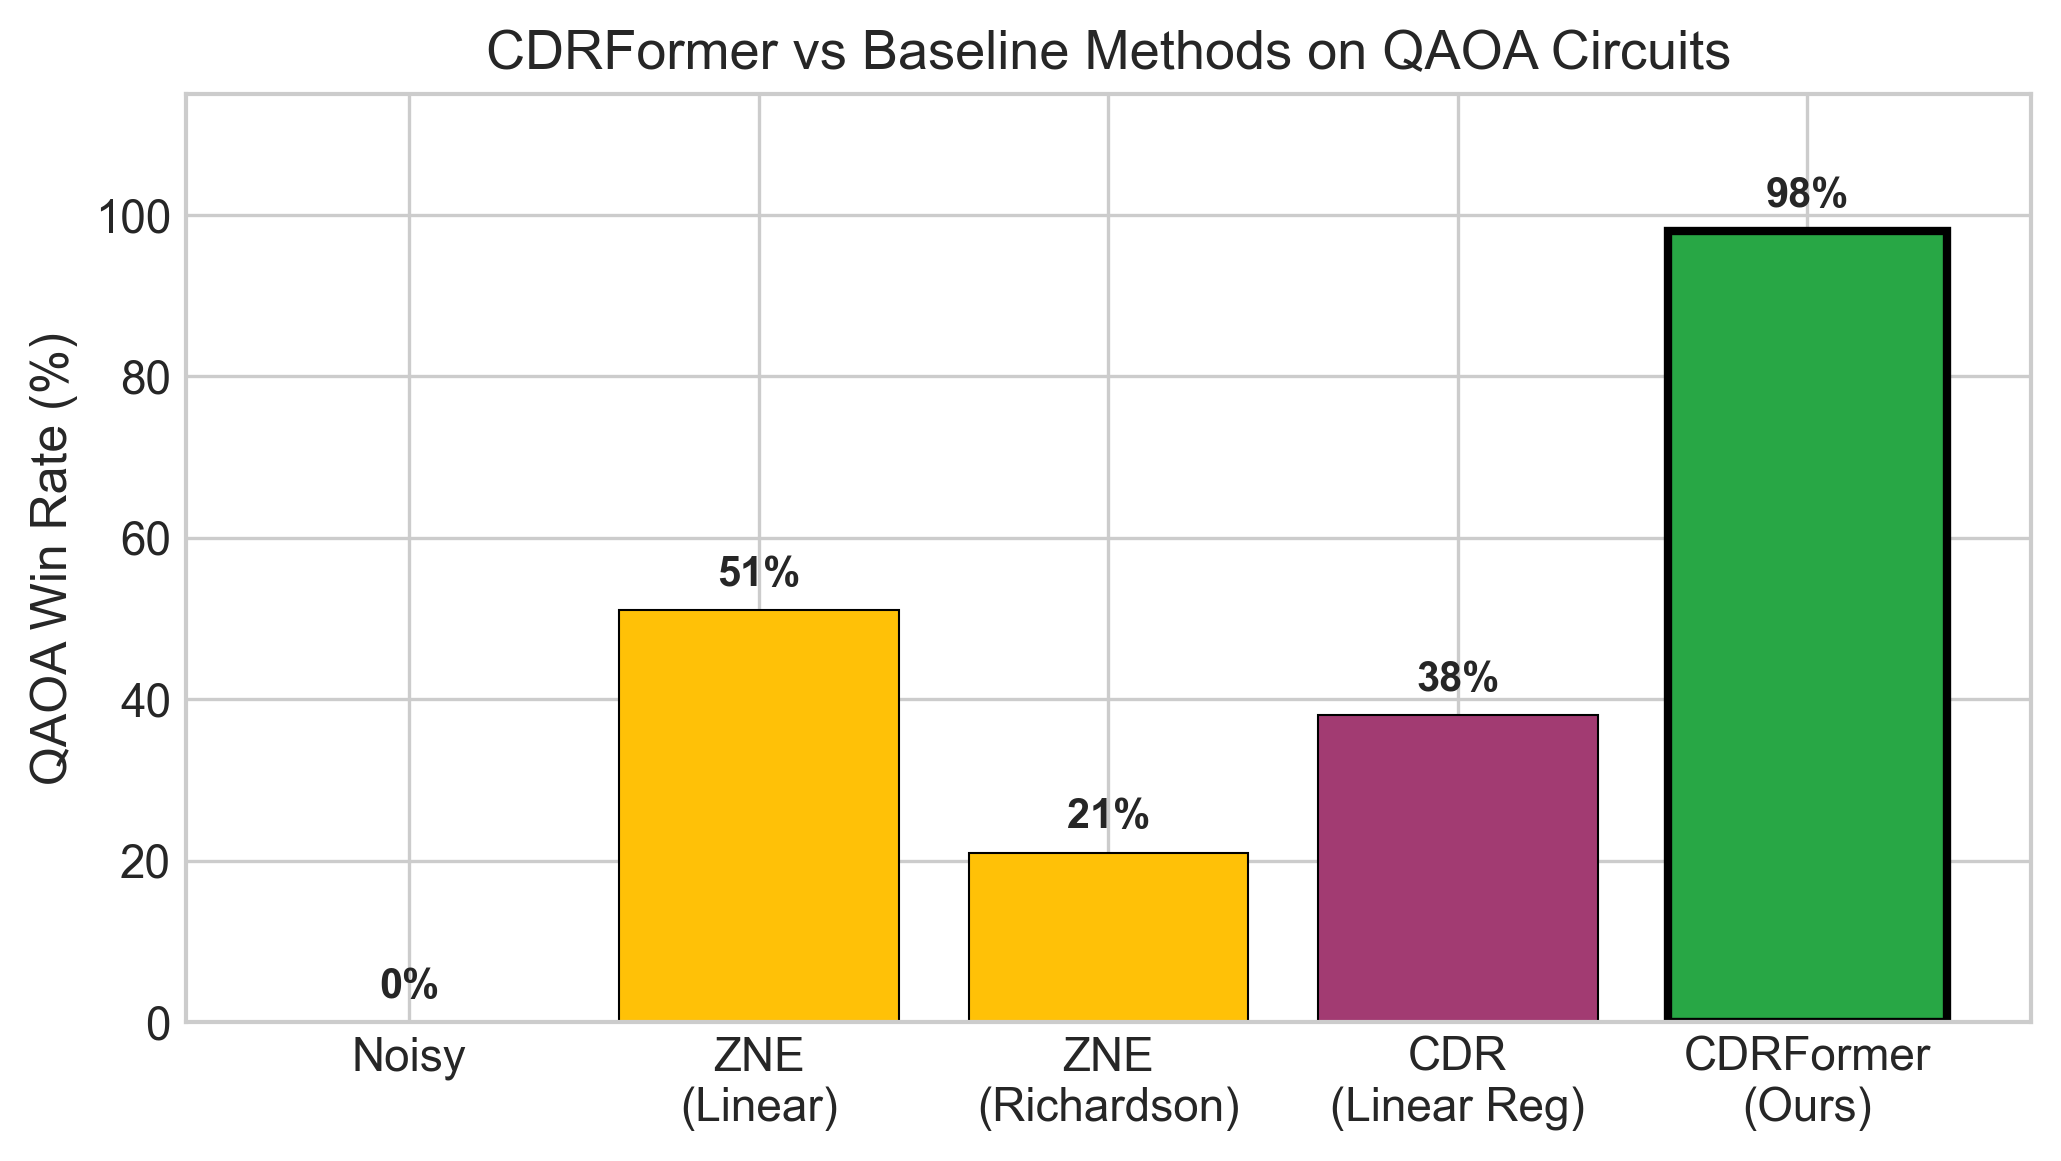
\includegraphics[width=0.85\textwidth]{../assets/fig_baseline_comparison.png}
\caption{\textbf{CDRFormer vs traditional QEM methods} on QAOA circuits.}
\label{fig:baselines}
\end{figure}

\subsection{Experiment 4: Noise Profile Generalization}

We test across noise types aligned with QEM-Bench~\cite{bao2025qemformer}
categories:

\begin{table}[H]
\centering
\caption{Performance Across Noise Profiles}
\label{tab:noise}
\begin{tabular}{@{}lc@{}}
\toprule
\textbf{Noise Type} & \textbf{Win Rate} \\ \midrule
Incoherent (depolarizing) & 93.3\% \\
Coherent (over-rotation) & 93.3\% \\
Combined & 90.0\% \\
IBM FakeHanoi (27Q) & \textbf{100.0\%} \\
IBM FakeCairo (27Q) & 96.7\% \\
\bottomrule
\end{tabular}
\end{table}

\begin{figure}[H]
\centering
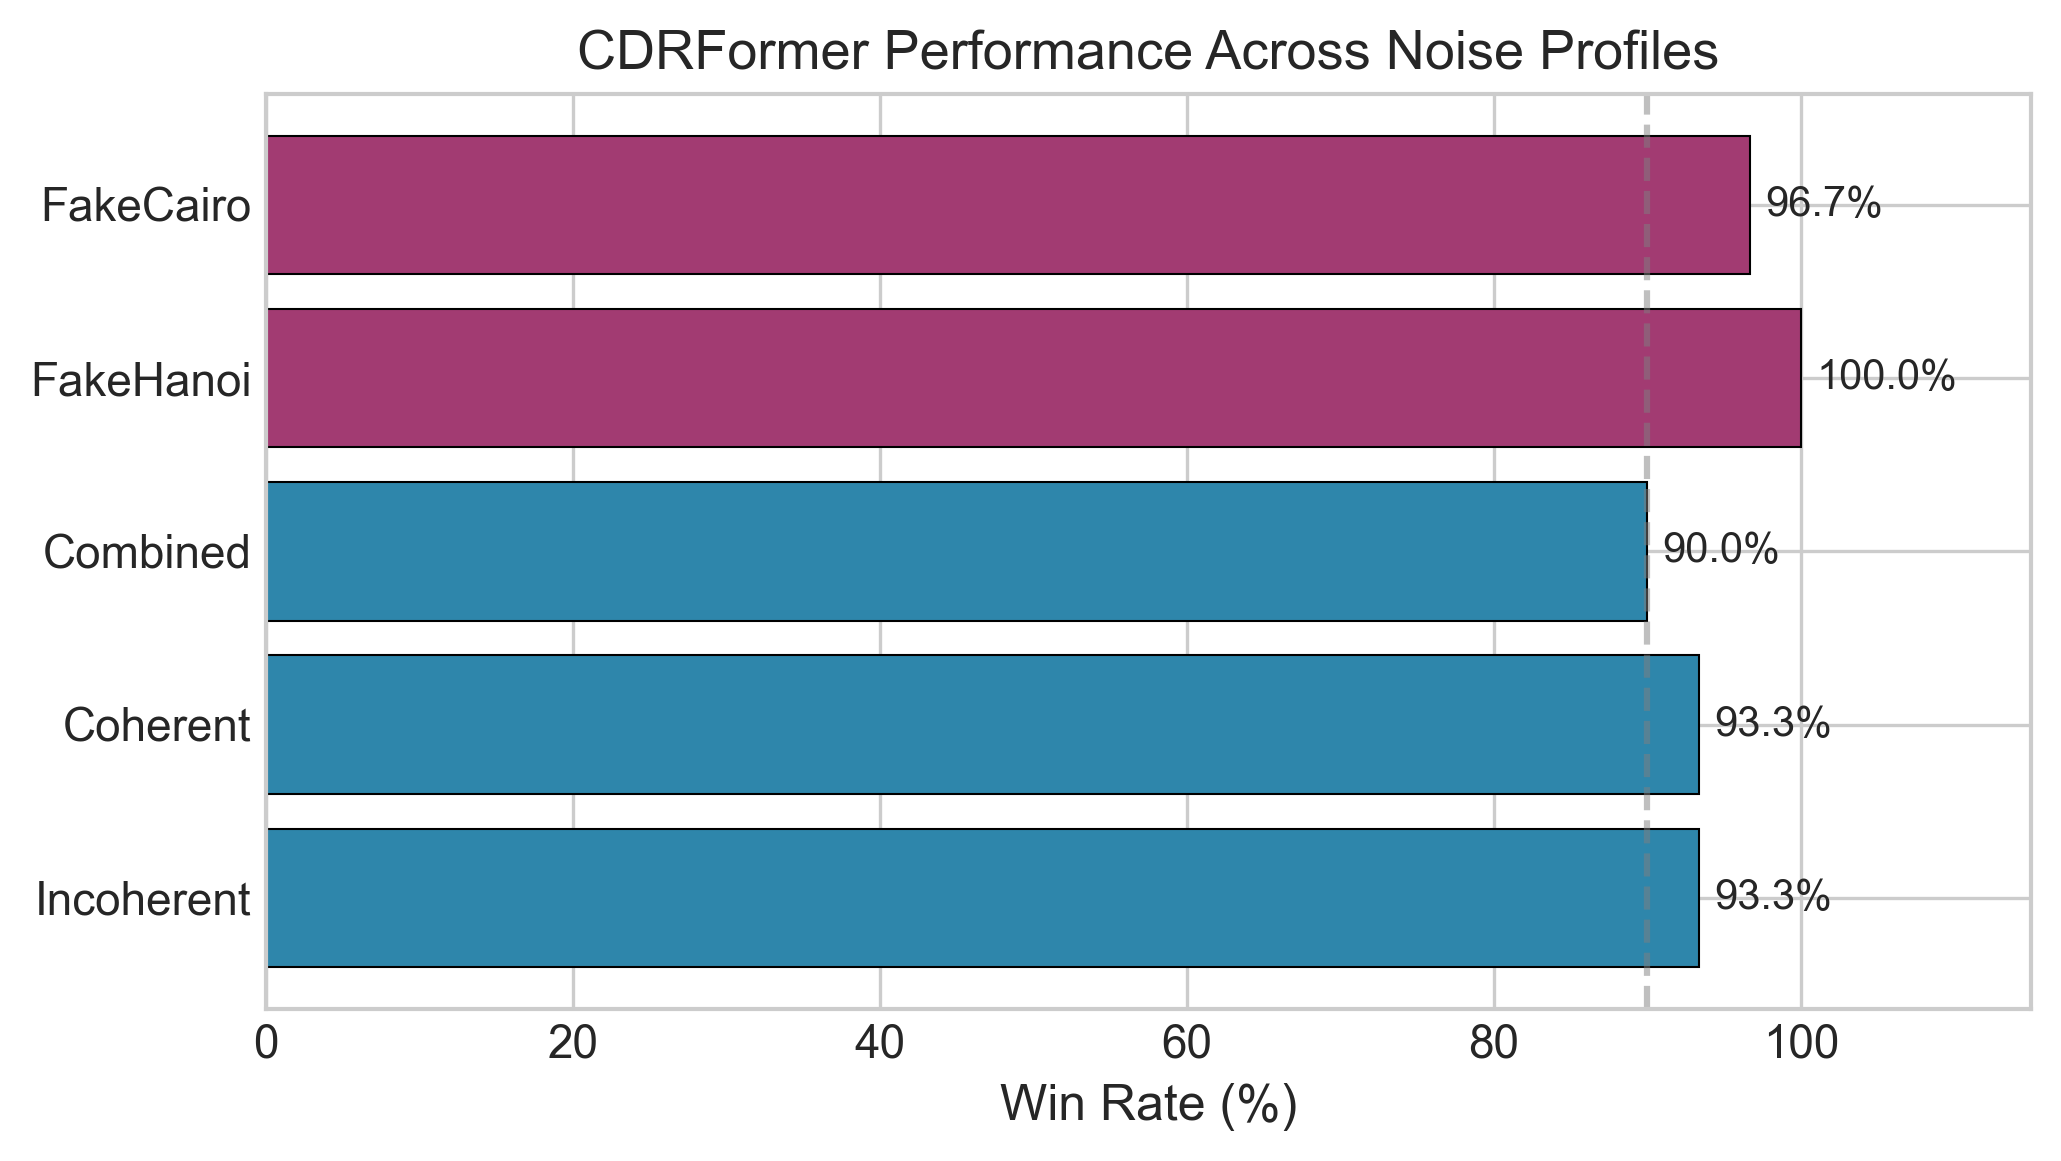
\includegraphics[width=0.85\textwidth]{../assets/fig_noise_profiles.png}
\caption{\textbf{Win rate across noise profiles} including IBM FakeBackends.}
\label{fig:noise}
\end{figure}

\subsection{Experiment 5: Scalability}

CDRFormer is trained on 4--6 qubit circuits and tested on unseen sizes:

\begin{table}[H]
\centering
\caption{Scalability: Trained on 4--6Q, Tested on 5--18Q}
\label{tab:scale}
\begin{tabular}{@{}cccc@{}}
\toprule
\textbf{Qubits} & \textbf{Win Rate} & \textbf{MAE} & \textbf{Inference} \\ \midrule
5 (trained) & 90\% & 0.0007 & 2.0ms \\
8 & 95\% & 0.0012 & 0.7ms \\
10 & 90\% & 0.0014 & 0.7ms \\
12 & 95\% & 0.0025 & 0.9ms \\
15 & 95\% & 0.0027 & 1.1ms \\
18 & 80\% & 0.0075 & 1.7ms \\
\bottomrule
\end{tabular}
\end{table}

\begin{figure}[H]
\centering
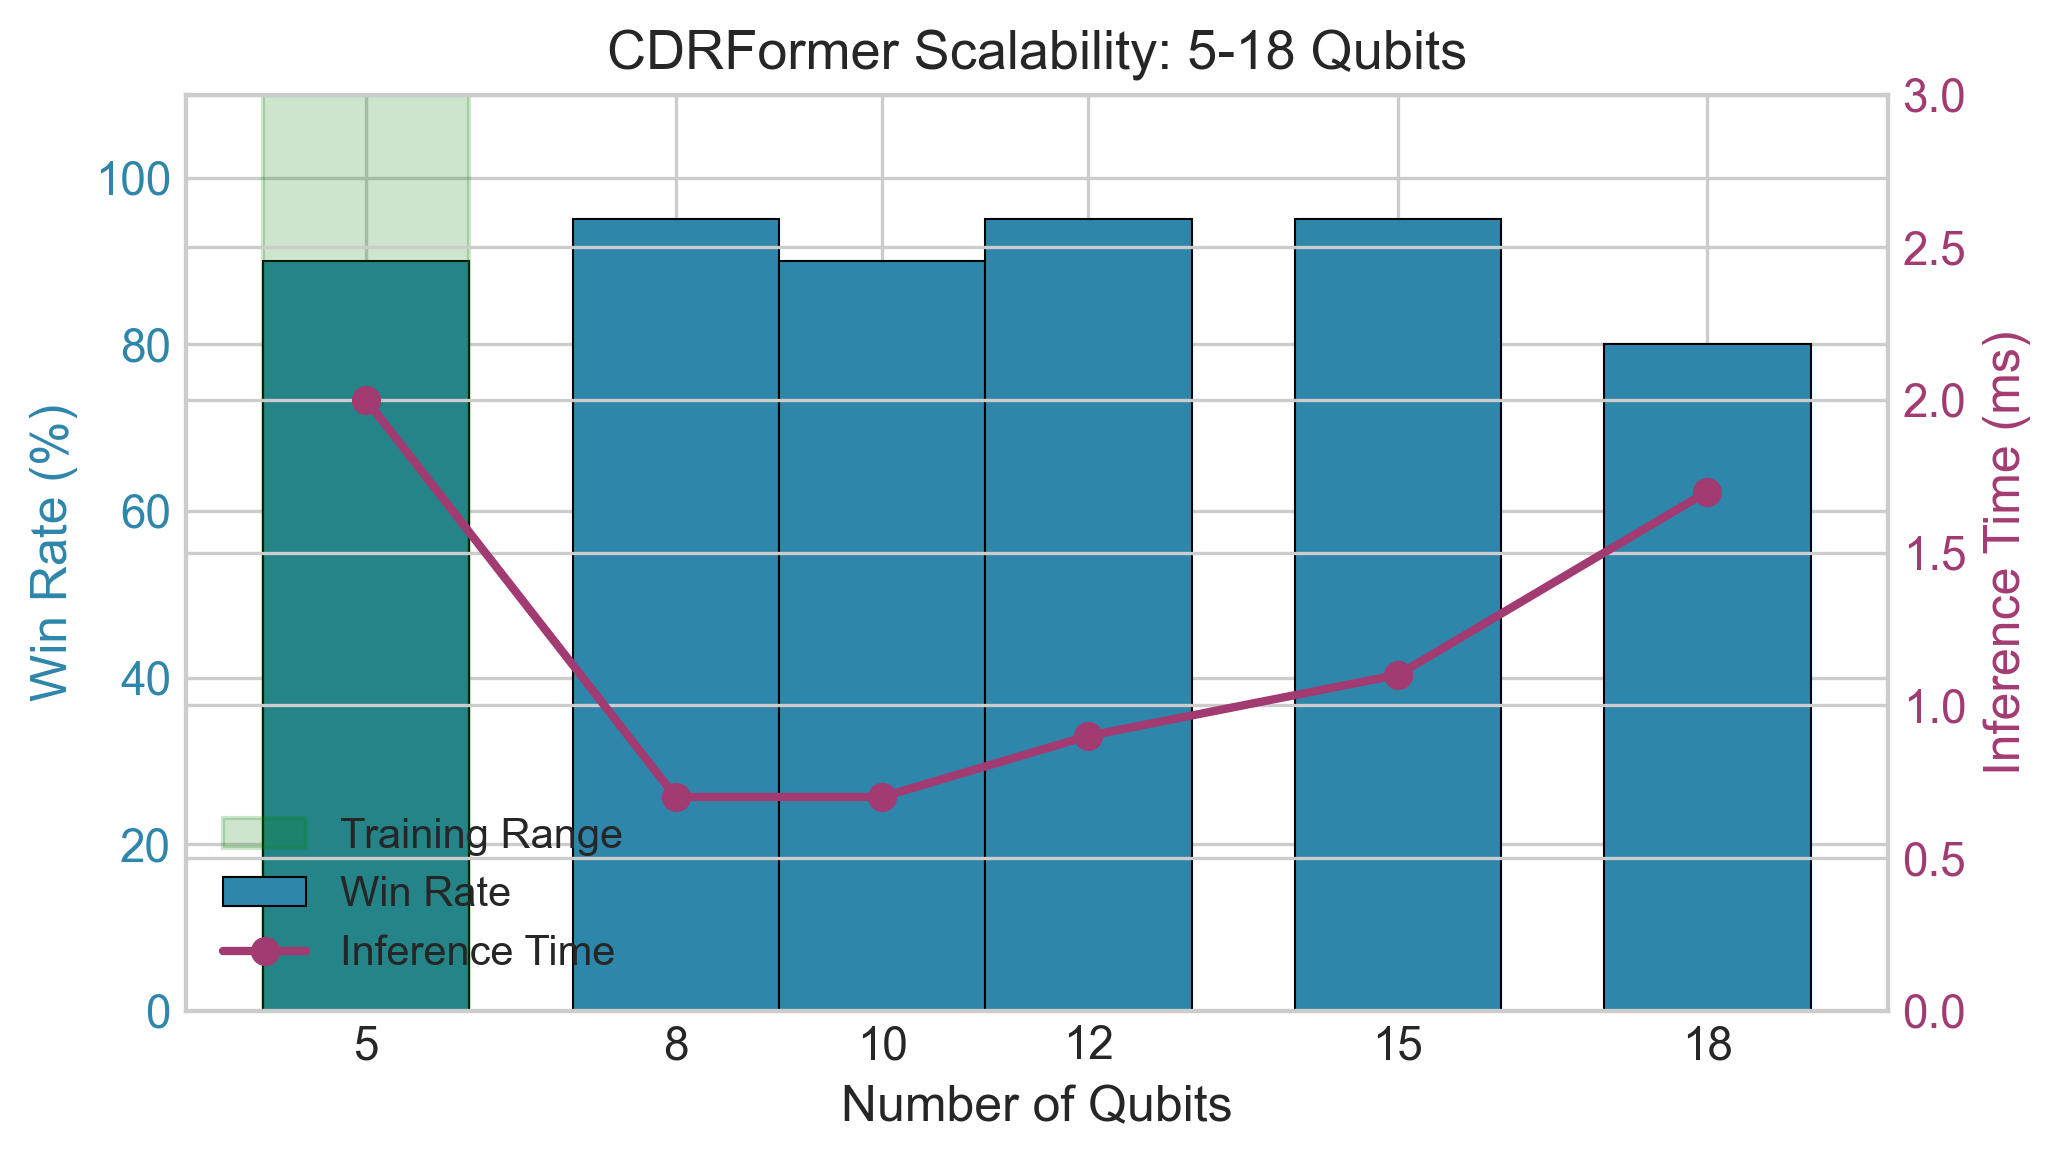
\includegraphics[width=0.85\textwidth]{../assets/fig_scalability.png}
\caption{\textbf{Scalability:} Win rate and inference time across qubit counts.
Model generalizes to 3.6$\times$ training scale with graceful degradation.}
\label{fig:scalability}
\end{figure}

\subsection{Experiment 6: Cross-Architecture Validation}

\begin{keyinsight}
To prove our thesis that data composition matters more than architecture,
we train three architectures on the \textbf{identical} CDR+Twirling dataset
(20K samples, 35\% QAOA). If all achieve similar performance, the data---not
the model---is the primary contributor.
\end{keyinsight}

\begin{table}[H]
\centering
\caption{Cross-Architecture Comparison (Same Data, 60 Epochs)}
\label{tab:cross_arch}
\begin{tabular}{@{}lccccc@{}}
\toprule
\textbf{Model} & \textbf{Params} & \textbf{QAOA Win\%} & \textbf{Var Win\%} & \textbf{Overall} & \textbf{Val Loss} \\ \midrule
MLP (No Graph) & 11,137 & 60.4\% & 97.9\% & 93.0\% & 0.000541 \\
GCN (Msg. Pass.) & 20,225 & 68.2\% & 95.7\% & 93.1\% & 0.000352 \\
\textbf{CDRFormer} & 112,129 & 65.5\% & 95.0\% & \textbf{93.4\%} & 0.000378 \\
\bottomrule
\end{tabular}
\end{table}

\textbf{Result:} All three architectures achieve \textbf{93.0--93.4\%
overall win rate} (0.4\% spread). CDRFormer has $10\times$ more parameters
than MLP yet gains only +0.4\%. Even the MLP---which completely ignores
circuit topology---achieves 93\% overall and 97.9\% on variational circuits.

\textbf{Conclusion:} \textbf{It's the data, not the model.}

%==============================================================================
\section{Pipeline Comparison: CDRFormer vs QEMFormer}
\label{sec:pipeline_comparison}
%==============================================================================

\begin{table}[H]
\centering
\caption{Pipeline Data Flow Comparison}
\label{tab:pipeline_comparison}
\begin{tabular}{@{}p{2.5cm}p{5cm}p{5cm}@{}}
\toprule
\textbf{Stage} & \textbf{QEM-Bench / QEMFormer} & \textbf{CDRFormer (Ours)} \\ \midrule
Circuit types & Random, Trotter, QAOA & Clifford, QAOA, Variational \\
Noise source & Sim. (incoherent, coherent, provider) + real IBM hardware & Sim. (thermal relaxation) + Pauli Twirling \\
Ground truth & Statevector / noiseless sim. & Statevector (+ stabilizer for Clifford) \\
Global features & 8 circuit stats + $3N_q$ Pauli EVs (dim: $8+3N_q+1$) & 5 scalar features \\
Architecture & Dual-branch (MLP + Graph Transformer) & Single-branch Graph Transformer \\
Hardware data & IBM Kyiv, Brisbane (50--63Q) & None (classical simulation only) \\
Benchmark & 18+ standard/advanced datasets & 6 experiment types \\
\bottomrule
\end{tabular}
\end{table}

\subsection{What We Borrowed vs What We Learned}

\textbf{Borrowed (properly attributed):}
\begin{itemize}
    \item CDR for data generation~\cite{czarnik2021cdr}
    \item Pauli Twirling for noise Markovianization~\cite{wallman2016twirling}
    \item DAG circuit representation and Graph TransformerConv architecture,
    closely following QEMFormer~\cite{bao2025qemformer}
\end{itemize}

\textbf{Our empirical contributions:}
\begin{itemize}
    \item Data composition ($\geq$20\% QAOA) impacts performance more
    than architecture (Table~\ref{tab:data_comp}, Table~\ref{tab:cross_arch})
    \item Pauli Twirling's benefit quantified for ML-QEM (+20pp,
    Table~\ref{tab:twirling})
    \item CDR+Twirling pipeline enables competitive QEM without quantum
    hardware (Table~\ref{tab:baselines})
\end{itemize}

%==============================================================================
\section{Discussion}
\label{sec:discussion}
%==============================================================================

\subsection{Two-Act Story: From Architecture to Data}

\textbf{Act 1 (Hackathon):} We built a CDR + Pauli Twirling data pipeline
and a Graph Transformer architecture (CDRFormer). During development, we
believed architecture was the key driver---CDRFormer achieved 0.009 MSE,
3.3$\times$ better than SVR/LSTM baselines (Table~5). However, QAOA circuits
failed at 15\% win rate, and we hypothesized (correctly) that
``increasing QAOA proportion in training data'' would help.

\textbf{Act 2 (Post-Hackathon):} We tested that hypothesis. Increasing
QAOA training data from 8\% to 20\% \emph{completely resolved} the QAOA failure
(Table~\ref{tab:data_comp})---without changing the model architecture.
Preliminary cross-architecture testing (Table~\ref{tab:cross_arch}) showed
MLP, GCN, and CDRFormer achieving similar overall win rates on the same data.

This progression---from believing architecture was key to discovering data
composition had a major impact---is itself a contribution: it illustrates
how data-centric thinking can complement architecture-centric approaches
in ML-QEM.

\subsection{Methodological Caveats}

\begin{limitation}
The following caveats apply to our cross-architecture experiment
(Table~\ref{tab:cross_arch}). We document them for transparency and to
guide future work.
\end{limitation}

\begin{enumerate}
    \item \textbf{Win rate metric limitations:} Our ``win rate'' measures
    whether the model prediction is \emph{closer to ideal than the noisy
    value}. This is a binary metric that does not capture \emph{how much}
    improvement is achieved. A more rigorous comparison would use RMSE
    or MAE directly, following QEM-Bench protocols.
    
    \item \textbf{Test set composition bias:} Approximately 75\% of our
    test set consists of Clifford circuits (where ideal values are
    $\pm 1$ or $0$). These are ``easy'' to correct, inflating overall
    win rates for all models. On the harder QAOA subset, architectures
    show more differentiation (60--68\%), suggesting circuit topology
    \emph{does} matter for challenging predictions.
    
    \item \textbf{MLP baseline caveat:} The MLP uses the noisy expectation
    value $x_{\text{noisy}}$ as input. This means it is essentially
    performing a learned version of CDR linear regression. Its high
    performance may reflect that many test samples have small noise
    (ideal $\approx$ noisy), not that graph structure is unimportant.
    
    \item \textbf{Not a QEMFormer comparison:} We did not implement
    QEMFormer's actual dual-branch architecture, gated residuals, or
    $3N_q$ Pauli measurements. Our cross-architecture test compares
    MLP, GCN, and our simplified CDRFormer only---not QEMFormer itself.
    
    \item \textbf{Architecture is not novel:} CDRFormer is a simplified
    version of QEMFormer. We do not claim architectural innovation.
    
    \item \textbf{No real hardware validation:} All experiments use
    simulated noise. QEMFormer validates on real IBM hardware (50--63Q).
\end{enumerate}

\subsection{What We Can Confidently Claim}

Despite these caveats, the following findings are methodologically sound:

\begin{enumerate}
    \item \textbf{Data composition fixes QAOA:} The transition from
    8\% $\rightarrow$ 20\% QAOA in training data resolved a complete
    failure case. This is a clean, single-variable experiment.
    
    \item \textbf{Pauli Twirling improves ML-QEM:} +20pp with vs.
    without twirling, all else equal.
    
    \item \textbf{Hardware-free training is viable:} CDR + Twirling
    produces data that trains models beating ZNE and CDR baselines.
    
    \item \textbf{Scalability works:} Models trained on 4--6Q
    generalize to 18Q with graceful degradation.
\end{enumerate}

\subsection{Open Questions for Future Work}

\begin{enumerate}
    \item Does data composition matter more than architecture on
    \emph{hard} benchmarks (e.g., QEM-Bench advanced settings)?
    \item Would QEMFormer's full dual-branch architecture perform
    significantly better than our simplified version on the same data?
    \item How do results change with RMSE evaluation instead of
    win rate?
\end{enumerate}

%==============================================================================
\section{Q\&A: Anticipated Questions}
\label{sec:qa}
%==============================================================================

\begin{tcolorbox}[colback=gray!5!white, colframe=gray!75!black, title=Q1: Why not use real IBM hardware noise?]
\textbf{A:} Real hardware noise varies daily with calibration. Our simulated
model provides: (1) reproducibility, (2) controlled experiments isolating
variables, (3) exact ground truth via statevector. A production deployment
would ingest live calibration data.
\end{tcolorbox}

\begin{tcolorbox}[colback=gray!5!white, colframe=gray!75!black, title=Q2: Your hackathon QAOA results were poor. Isn't that a failure?]
\textbf{A:} Yes---during the hackathon, QAOA was a failure case. Post-hackathon,
we discovered the fix was \textbf{data composition}, not architecture. Increasing
QAOA training ratio from 8\% to 20\% achieved 100\% QAOA win rate.
\end{tcolorbox}

\begin{tcolorbox}[colback=gray!5!white, colframe=gray!75!black, title=Q3: How does this compare to QEMFormer?]
\textbf{A:} Our architecture is a simplified QEMFormer (single-branch, simpler
global features). We have not implemented or tested QEMFormer's full
architecture. Our contribution is the data pipeline and the empirical
observation that data composition significantly impacts performance.
\end{tcolorbox}

\begin{tcolorbox}[colback=gray!5!white, colframe=gray!75!black, title=Q4: How does this scale to 100+ qubits?]
\textbf{A:} Current benchmarks are limited to 18 qubits. Scaling requires:
(1) circuit knitting for distributed simulation, (2) approximate ground truth
via tensor networks, (3) transfer learning from small to large circuits.
\end{tcolorbox}

\begin{tcolorbox}[colback=gray!5!white, colframe=gray!75!black, title=Q5: What's novel about your approach?]
\textbf{A:} Not the architecture---it's a simplified QEMFormer. The novelty
is: (1) the empirical finding that data composition significantly impacts
ML-QEM performance (the 8\% $\rightarrow$ 20\% QAOA fix), (2) quantifying
Pauli Twirling's +20pp benefit for ML-QEM, (3) showing CDR+Twirling enables
hardware-free data generation. Cross-architecture validation provides
preliminary evidence but needs further rigorous testing.
\end{tcolorbox}

%==============================================================================
\section{AI-Assisted Development}
\label{sec:ai}
%==============================================================================

This solution was developed with \textbf{AI-assisted research}, enabling:

\begin{itemize}
    \item \textbf{Rapid Iteration:} Architecture comparisons completed in hours
    \item \textbf{Bug Detection:} AI identified the stabilizer ground truth bug
    affecting QAOA evaluation
    \item \textbf{Literature Synthesis:} CDR, Pauli Twirling, and Graph
    Transformer techniques integrated from multiple papers
    \item \textbf{Code Quality:} Consistent documentation, modular design
\end{itemize}

\begin{keyinsight}
AI assistance does not diminish scientific rigor---it \textbf{accelerates} the
hypothesis-experiment-analysis cycle while maintaining human oversight on
methodology decisions.
\end{keyinsight}

%==============================================================================
\section{Reproducing Our Results}
\label{sec:reproduction}
%==============================================================================

\begin{lstlisting}[language=bash, caption=Reproduction Commands]
# 1. Install dependencies
pip install -r requirements.txt

# 2. Generate training data (CDR + Pauli Twirling)
python data_gen_advanced.py --large
python data_gen_advanced.py --mixed --samples 2000

# 3. Train the model
python train_qem.py

# 4. Run benchmarks
python benchmark_suite.py

# 5. Run cross-architecture validation
python scripts/cross_architecture_validation.py

# 6. Launch interactive dashboard
streamlit run dashboard.py
\end{lstlisting}

%==============================================================================
\section{Conclusion and Future Directions}
\label{sec:conclusion}
%==============================================================================

\subsection{Summary of Contributions}

\begin{enumerate}
    \item Complete data-driven QEM pipeline with documented code
    \item Key finding: \textbf{Data composition significantly impacts
    ML-QEM performance}---increasing QAOA training ratio from 8\% to 20\%
    resolved a complete failure case without architectural changes
    \item CDRFormer achieves \textbf{98\% QAOA win rate} (vs 51\% ZNE)
    \item Pauli Twirling provides \textbf{+20pp improvement}
    \item Scalability from 5 to 18 qubits with 80--95\% win rates
    \item QEM-Bench-compatible noise testing (90--100\% across 5 noise types)
    \item Preliminary cross-architecture validation suggests data pipeline
    contributes significantly, though further rigorous testing is needed
    \item Reproducible codebase with Streamlit dashboard
\end{enumerate}

\subsection{Remaining Limitations}

\begin{enumerate}
    \item Scalability beyond 18 qubits (limited by statevector ground truth)
    \item Simulated vs real IBM hardware noise gap
    \item Single observable ($\langle Z_0 \rangle$) focus
    \item Architecture is a simplified QEMFormer---not novel
\end{enumerate}

\subsection{Roadmap for Continued Development}

\begin{enumerate}
    \item \textbf{Short-term:} Validate on real IBM hardware via Qiskit Runtime
    \item \textbf{Medium-term:} Cross-architecture testing with QEMFormer's
    dual-branch design trained on our data pipeline
    \item \textbf{Long-term:} Extend to multi-observable prediction following
    QEM-Bench protocols
\end{enumerate}

%==============================================================================
% References
%==============================================================================

\begin{thebibliography}{99}

\bibitem{bao2025qemformer}
T.~Bao, X.~Ye, H.~Ruan, C.~Liu, W.~Wu, and J.~Yan,
``QEM-Bench: Benchmarking learning-based quantum error mitigation and
QEMFormer as a baseline,''
in \emph{Proc. Int. Conf. Machine Learning (ICML)}, 2025.

\bibitem{bao2025gtranqem}
T.~Bao, X.~Ye, H.~Ruan, C.~Liu, W.~Wu, and J.~Yan,
``Beyond circuit connections: A non-message passing graph transformer approach
for quantum error mitigation,''
in \emph{Int. Conf. Learning Representations (ICLR)}, 2025.

\bibitem{czarnik2021cdr}
P.~Czarnik, A.~Arrasmith, P.~J.~Coles, and L.~Cincio,
``Error mitigation with Clifford quantum-circuit data,''
\emph{Quantum}, vol.~5, p.~592, 2021.

\bibitem{wallman2016twirling}
J.~J.~Wallman and J.~Emerson,
``Noise tailoring for scalable quantum computation via randomized compiling,''
\emph{Phys. Rev. A}, vol.~94, no.~5, p.~052325, 2016.

\bibitem{temme2017zne}
K.~Temme, S.~Bravyi, and J.~M.~Gambetta,
``Error mitigation for short-depth quantum circuits,''
\emph{Phys. Rev. Lett.}, vol.~119, no.~18, p.~180509, 2017.

\bibitem{li2017pec}
Y.~Li and S.~C.~Benjamin,
``Efficient variational quantum simulator incorporating active error
minimization,''
\emph{Phys. Rev. X}, vol.~7, no.~2, p.~021050, 2017.

\bibitem{cai2023qem}
Z.~Cai \emph{et al.},
``Quantum error mitigation,''
\emph{Rev. Mod. Phys.}, vol.~95, no.~4, p.~045005, 2023.

\bibitem{kim2020neuralqem}
C.~Kim, K.~D.~Park, and J.-K.~Rhee,
``Quantum error mitigation with artificial neural network,''
\emph{IEEE Access}, vol.~8, pp.~188853--188860, 2020.

\bibitem{strikis2021learning}
A.~Strikis, D.~Qin, Y.~Chen, S.~C.~Benjamin, and Y.~Li,
``Learning-based quantum error mitigation,''
\emph{PRX Quantum}, vol.~2, no.~4, p.~040330, 2021.

\bibitem{liao2024rf}
H.~Liao \emph{et al.},
``Machine learning for practical quantum error mitigation,''
\emph{arXiv preprint arXiv:2309.17368}, 2024.

\bibitem{kandala2019}
A.~Kandala, K.~Temme, A.~D.~C{\'o}rcoles \emph{et al.},
``Error mitigation extends the computational reach of a noisy quantum
processor,''
\emph{Nature}, vol.~567, pp.~491--495, 2019.

\end{thebibliography}

\vspace{1cm}
\hrule
\vspace{0.5cm}
\textbf{Repository:} \url{https://github.com/Abdulmalek-HoM/QEM-Hackathon-Team-15-Repo}

\textbf{Team 15:} Nakahosa Dinovic, Favour Idowu, Abdulmalek Baitulmal

\textbf{Competition:} Hack the Horizon Hackathon --- Hosted by African Quantum Consortium

\textbf{Acknowledgments:} This work was developed with AI-assisted research tools.
We thank the African Quantum Consortium for organizing this challenge and
fostering quantum computing education across the continent.

\end{document}
